\documentclass[hyperref, UTF8, a4paper]{ctexart}

\usepackage{geometry}
\usepackage{titling}
\usepackage{titlesec}
\usepackage{paralist}
\usepackage{footnote}
\usepackage{enumerate}
\usepackage{amsmath, amssymb, amsthm}
\usepackage{bbm}
\usepackage{cite}
\usepackage{graphicx}
\usepackage{subfigure}
\usepackage{physics}
\usepackage{tensor}
\usepackage{tikz}
\usepackage{tikz-feynhand}
\usepackage[colorlinks, linkcolor=black, anchorcolor=black, citecolor=black]{hyperref}
\usepackage{prettyref}
\usepackage{extarrows}

\usepackage[inkscapearea=page]{svg}

\geometry{left=3.18cm,right=3.18cm,top=2.54cm,bottom=2.54cm}
\titlespacing{\paragraph}{0pt}{1pt}{10pt}[20pt]
\setlength{\droptitle}{-5em}
\preauthor{\vspace{-10pt}\begin{center}}
\postauthor{\par\end{center}}

\DeclareMathOperator{\timeorder}{T}
\DeclareMathOperator{\diag}{diag}
\DeclareMathOperator{\legpoly}{P}
\DeclareMathOperator{\primevalue}{P}
\DeclareMathOperator{\sgn}{sgn}
\newcommand*{\ii}{\mathrm{i}}
\newcommand*{\ee}{\mathrm{e}}
\newcommand*{\const}{\mathrm{const}}
\newcommand*{\comment}{\paragraph{注记}}
\newcommand*{\suchthat}{\quad \text{s.t.} \quad}
\newcommand*{\argmin}{\arg\min}
\newcommand*{\argmax}{\arg\max}
\newcommand*{\normalorder}[1]{: #1 :}
\newcommand*{\pair}[1]{\langle #1 \rangle}
\newcommand*{\fd}[1]{\mathcal{D} #1}

\newrefformat{sec}{第\ref{#1}节}
\newrefformat{note}{注\ref{#1}}
\newrefformat{fig}{图\ref{#1}}
\renewcommand{\autoref}{\prettyref}

\usetikzlibrary{arrows,shapes,positioning}
\usetikzlibrary{arrows.meta}
\usetikzlibrary{decorations.markings}
\tikzstyle arrowstyle=[scale=1]
\tikzstyle directed=[postaction={decorate,decoration={markings,
    mark=at position .5 with {\arrow[arrowstyle]{stealth}}}}]
\tikzstyle ray=[directed, thick]
\tikzstyle dot=[anchor=base,fill,circle,inner sep=1pt]

\renewcommand{\emph}[1]{\textbf{#1}}
\newcommand*{\concept}[1]{\underline{\textbf{#1}}}

\title{相对论}
\author{吴晋渊}

\begin{document}

\maketitle

\section{狭义相对论的时空观}

\subsection{狭义相对论的导出}

\subsubsection{时空,世界线和参考系}

我们的世界有三个空间维和一个时间维。牛顿时空观下,时间维和空间维没有什么关系:不管怎么做伽利略变换,时间维都不会发生什么变化。
这个图像在麦克斯韦方程组出现之后受到了很大挑战,因为后者并不具有伽利略不变性。相反,存在一个和参考系无关的连接时间和空间的常数:光速。
对让麦克斯韦方程组不变的参考系变换的探索最终导致了狭义相对论。
本节将从一些看起来十分合理的基本原理出发,导出狭义相对论。

我们认为时空流形中的点标记了\concept{事件},即一个事件可以完全通过“某个时间点,某个空间点发生了一些事情”来描述。
我们暂时只讨论经典情况,这样一个系统中就会有可以用一个完全确定的位置(它是$\mathbb{R}^3$中的点)标记的“粒子”或者“信号”%
\footnote{什么是粒子其实是需要手动指定的。可以想象非常远的距离的两端依次发生了两个事件,但这并不代表有什么东西从这段距离的一端传到了另一端。
一个其坐标出现在动力学方程中的“东西”显然是一个粒子,空间中的场的可以连续传播的构型的“位置”或许也可以看成一个粒子或者说信号。
}%
。
这就是粒子自由度。当然其实还有场自由度,我们一般确信,场的小幅扰动给出某种粒子(经典情况下是波包,量子情况下可以做二次量子化),从而,虽然“坐标”对粒子自由度和场自由度的意义是不同的——在前者中坐标是直接出现在运动方程中的待求解的量,在后者中坐标只是时空点的标记,提供一个背景——粒子的坐标和场的坐标在同一个时空流形中,两者是同一种东西。
我们可以通过分析粒子的坐标需要满足的性质得到时空的几何结构,然后在此之上分析场的运动。

我们认为只有一个时间维,因此每个粒子的历史就构成了一个\concept{世界线},一个世界线由一系列排成一排的事件组成。
世界线当然可以被参数化,我们认为有某种普适的、不依赖于坐标的方法——所谓\concept{固有时}——可以标记任何一条世界线上各个事件的时间,即可以给任意一段世界线指派一个坐标无关的、可加的实数。

事件当然可以被观察到。我们如果要记录一个事件,肯定是设立一些“观测点”,这些观测点在某个时间点的空间位置是确定的,我们让时间演化并同时“看表”(或者说检查观测点的固有时),如果某个观测点附近(一定要是附近,因为我们要求相互作用具有局域性)发生了某个事件,我们就记录下来了这个事件。
因此,很自然地,我们应该能够用一族观察者的世界线以及这些时间线上的固有时标记任何一个事件(既然任何事件都应该能被一些人观测到)。
我们称一族观察者组成\concept{参考系},当且仅当,对时空中每一点,有且只有一个观察者的世界线通过它。
参考系中这些世界线的固有时自然地给出了参考系中的时间坐标的坐标线,与这些坐标线垂直的坐标线则给出了空间坐标。
显然,沿着构成参考系的观察者世界线走,空间坐标是不会变的,因此选定参考系等价于选定“什么是静止的”。
有坐标系就可以定义一个参考系,有参考系并结合上适当的空间坐标选取(只需要满足空间坐标的坐标线和时间坐标的坐标线垂直即可)就可以定义坐标系。
% TODO:局域的?

以上的定义都只是在写下我们对时空的直觉,下面我们开始讨论狭义相对论特有的假设。

\subsubsection{狭义相对性原理}

狭义相对论包括下面的基本假设:
\begin{itemize}
    \item 一些常见的隐含假设:所有物理定律都满足空间均匀、各向同性的条件,时间平移不变性成立。
    特别的我们还认为空间就是均匀的$\mathbb{R}^3$。
    这意味着在选定一个坐标系之后,我们可以对一条世界线定义\concept{匀速直线运动}等概念——实际上,我们还可以将匀速直线运动当成一种从一个参考系切换到另一个参考系的操作。
    \item \concept{狭义相对性原理},具体来说:
    \begin{itemize}
        \item 对任意一个时空点$p$,都存在一个其世界线通过$p$的\concept{惯性观测者}$O$,一个惯性观测者经过空间平移之后覆盖整个时空而得到的参考系称为\concept{惯性参考系},在其中$O$是静止的。%
        \footnote{
            到这里我们还没有选取空间坐标,但是因为我们已经假定空间就是$\mathbb{R}^3$,其实随便选一个直角坐标系就可以。
        }% 
        并且任何两个惯性观测者世界线都可以通过空间平移(由于空间均匀,并无定义问题)、时间平移(由于曲线参数可以随意选取,也没有定义问题)、空间和时间的伸缩和匀速直线运动%
        \footnote{
            说得更加明确一些,设$O$是惯性观测者,使用$O$确定的参考系中的世界线如果满足$\vb*{x}(t) = \vb*{x}_0 + \vb*{u} t$,那么我们认为这条世界线确定了另外一个惯性观测者。
            显然,匀速直线运动还确定了两个惯性参考系之间的变换。
        }%
        来相互转化。
        
        容易看出惯性参考系之间差一个整体的空间平移或是匀速直线运动%
        \footnote{
            需要注意的是,设惯性参考系$S'$中的某个静止点在惯性参考系$S$中的坐标为$\vb*{x}$,则必然有$\vb*{x} = \vb*{x}_0 + \vb*{u} t$,但是没有什么理由让我们认为$S$系和$S'$系之间的坐标变换也是这个形式——实际上,到现在为止我们连$S$系和$S'$系之间的坐标变换是不是仿射变换都不知道!
            我们在这里要求的仅仅是存在性,即从一个惯性参考系和一个在这个惯性参考系中的匀速直线运动出发总是可以得到另一个惯性参考系。
        }%
        ,并且在任意的惯性参考系中,一条惯性观测者时间线都是匀速直线运动,匀速直线运动的粒子也构成惯性观测者。这又意味着,在一个惯性参考系中看来是在做匀速直线运动的粒子在任何惯性参考系中都在做匀速直线运动,因为一个世界线是不是惯性观测者的世界线和参考系无关。
        反之,如果一个参考系$S$中有惯性观测者在做匀速直线运动,那么这个参考系也是惯性参考系,因为可以从$S$做一个匀速直线运动得到一个惯性参考系,因此$S$也是一个惯性参考系。%
        \footnote{
            然而应当注意,由于我们要求参考系的时间坐标线和空间坐标线垂直,虽然我们总是可以对一个惯性参考系的坐标做一个线性变换而让原本是匀速直线运动的世界线保持匀速直线运动,但是这样得到的新坐标系可能不再是一个良好的“参考系”了。
            要确定什么是“垂直”我们需要度规,而我们马上可以看到,正是光速不变原理给出了度规。
        }%

        以上假设基本上继承了伽利略时空观。
        \item 不同惯性参考系中的物理规律(或者说,用不同的惯性参考系的坐标表述的物理规律)形式相同。这个假设也是伽利略时空观中有的。
        这意味着没有一个物理过程能够说出“我们在哪个参考系内”——参考系只是可以更换的标签。
    \end{itemize}
    \item \concept{光速不变原理}:有某种运动的速度%
    \footnote{
        一个参考系中的事件传播速度就是空间变化除以时间变化,这点在狭义相对论中是保持的。我们要求这两个事件在一条世界线上,否则“速度”的概念缺乏意义,因为此时并没有什么东西实际上被传递了。
    }%
    在不同的惯性参考系中都是一样的,这个速度称为\concept{光速}。
    “光速”一词来自波动方程中的光速在参考系变换下不变这一事实,不过在这里我们暂时将它作为一个无意义的名词使用;实际上,狭义相对论中光速的作用在于在时间和空间之间建立关系。
    
    这个假设对惯性系做了额外的限制,正是这个假设让狭义相对论和伽利略时空观完全不同。
    我们将看到,光速不变原理实际上给出了一个四维时空中的度规。
\end{itemize}

惯性参考系可以在时间和空间上无限平移意味着我们在处理$\mathbb{R}^4$。
考虑两个惯性参考系$S$和$S'$,分别用$(t, x, y, z)$和$(t', x', y', z')$标记其中的事件。
设一个信号以光速运动,它某时刻在某地出现,记作事件$P_1$,另一时刻在另一地点出现,记作事件$P_2$。
$P_1$和$P_2$在这个信号的世界线上,其速率为光速,其运动方向保持不变,于是我们可以简单地用勾股定理得到
\[
    (x_1 - x_2)^2 + (y_1 - y_2)^2 + (z_1 - z_2)^2 = c^2 (t_1 - t_2)^2, 
\]
以及
\[
    (x_1' - x_2')^2 + (y_1' - y_2')^2 + (z_1' - z_2')^2 = c^2 (t_1' - t_2')^2.
\]
在这里,光速不变性的不同寻常之处已经可以体现出来了:如果我们朴素地做伽利略变换,设$S'$系相对$S$以速度$u$沿着$x$轴运动,则
\[
    x_1' = x_1 + u t_1, \quad x_2' = x_2 + u t_2,
\]
于是
\[
    (x_1 - x_2 + u t_1 - u t_2)^2 - (x_1 - x_2)^2 = c^2 (t_1' - t_2')^2 - c^2 (t_1 - t_2)^2,
\]
因此
\[
    (t_1' - t_2')^2 \neq (t_1 - t_2)^2.
\]
这意味着两个参考系中时间流动的速率不一样,就导出了一个矛盾。因此满足光速不变性的参考系变换肯定不是伽利略变换。

简而言之,如果一个信号以光速运动,那么在任何参考系中都有
\[
    c^2 (t_1 - t_2)^2 - (x_1 - x_2)^2 - (y_1 - y_2)^2 - (z_1 - z_2)^2 = 0.    
\]
反之,如果某个参考系中有上式成立,那么信号一定以光速运动。于是我们定义两个事件的\concept{间隔}为
\begin{equation}
    s^2 = c^2 (t_1 - t_2)^2 - (x_1 - x_2)^2 - (y_1 - y_2)^2 - (z_1 - z_2)^2,
\end{equation}
并且如果一个参考系中的间隔为零,那么别的参考系中的间隔也为零。

现在我们考虑靠得很近的两个事件,即考虑$\dd{s^2}$。坐标变换是连续的,即$\dd{s^2}$和$\dd{s'^2}$是同阶小量,并且$\dd{s^2}=0$时$\dd{s'^2}=0$。
因此我们设
\[
    \dd{s^2} = a \dd{s'^2}.
\]
现在再引入一个惯性参考系$S''$。由空间的均匀性和各向同性,$a$不应该显含任何坐标,无论是时间还是空间,因此它只应该依赖于两个惯性参考系之间的相对速度(我们不能预期$S$在$S'$中的运动速度和$S'$在$S$中的运动速度只差一个负号,但是它们之间显然是有关系的),而且不能依赖于相对速度的方向。
设$S'$在$S$中的运动速度大小为$V_1$,$S''$在$S$中的运动速度大小为$V_2$,$S''$在$S'$中的运动速度为$V_3$,则显然
\[
    \dd{s'^2} = a(V_1) \dd{s^2}, \quad \dd{s''^2} = a(V_2) \dd{s^2}, \quad \dd{s''^2} = a(V_3) \dd{s'^2},
\]
于是
\[
    a(V_3) = \frac{a(V_1)}{a(V_2)}.
\]
但是$V_3$不仅依赖于$V_1$和$V_2$,肯定还依赖于它们的相对角度,而上式右边却没有出现任何相对角度,因此仅有的可能是$a$根本就是一个常数,代入上式就有$a = 1$,于是
\begin{equation}
    \dd{s^2} = \dd{s'^2},
\end{equation}
即时空间隔在不同的惯性参考系中完全一样。

\subsubsection{四维闵可夫斯基时空和洛伦兹变换}

在重新定义时间的单位,从而用$t$代替$ct$之后,我们就得到
\begin{equation}
    \dd{s}^2 = \dd{t}^2 - \dd{x}^2 - \dd{y}^2 - \dd{z}^2,
\end{equation}
并且这个量在不同惯性参考系中保持不变。
于是,在任意的惯性参考系中,我们附加一个度规
\begin{equation}
    [\eta_{\mu \nu}]_{\mu \nu} = \diag{(1, -1, -1, -1)},
    \label{eq:min-metrics}
\end{equation}
就会发现不同惯性参考系实际上描述了同一个\concept{四维闵可夫斯基时空}——即$(\mathbb{R}^4, \eta_{ab})$。正是光速不变原理给出了闵可夫斯基度规。
闵可夫斯基时空是平直的。注意到$(\mathbb{R}^4, \eta_{ab})$中$\partial_a \eta_{bc} = 0$,因此$\partial_a$就是$\nabla_a$。

如果一个参考系是惯性参考系,那么其中的度规就是\eqref{eq:min-metrics}。
惯性系之间的坐标变换在忽略了平移之后就是一个矩阵群,称为\concept{洛伦兹变换}。
洛伦兹变换保持度规分量始终为\eqref{eq:min-metrics}。
全体保度规变换组成的群的李代数由Killing矢量场给出。计算可以发现以下矢量场是Killing场:
\begin{itemize}
    \item 与平移相关的四个Killing矢量场$(\partial_\mu)^a$,
    \item 与旋转相关的三个Killing矢量场$-y (\partial_x)^a + x (\partial_y)^a$,$-z (\partial_y)^a + y (\partial_z)^a$和$-x (\partial_z)^a + z (\partial_x)^a$,
    \item 和推动(boost,即两个差一个匀速直线运动的参考系之间的变换)相关的$t (\partial_i)^a + x_i (\partial_t)^a$。
\end{itemize}
我们已经找到10个独立Killing矢量场了,而最多也就只有$4(4+1)/2=10$个Killing矢量场,因此我们已经找到了所有的Killing矢量场,且发现闵可夫斯基时空的对称性是很高的。
注意到,除了平移以外的Killing矢量场诱导出的坐标变换都是线性的,从而一个惯性坐标系经过保度规变换之后得到的坐标系中,所有惯性观测者都做匀速直线运动。
另一方面,由度规\eqref{eq:min-metrics}的含义,光速不变性在保度规变换之后还是成立的。
因此全体保度规变换都是惯性参考系之间的变换。因此,洛伦兹变换实际上就是全体保度规变换,即洛伦兹群实际上给出了$(\mathbb{R}^4, \eta_{ab})$在排除平移后的时空对称性。

在找到一个惯性参考系之后,适当作用平移和洛伦兹变换——这两种操作构成\concept{庞加莱群}——就得到了所有惯性参考系。
容易看出,庞加莱群给出了$(\mathbb{R}^4, \eta_{ab})$的完整的时空对称性。

我们现在来看看洛伦兹群的群元有哪些。与旋转相关的那三个Killing矢量场实际上只是把空间坐标轴转了一下,可以说只是改变了惯性坐标系,但是没有实质性地改变惯性参考系。
推动才是真正改变了惯性参考系的操作。不失一般性地考虑$t (\partial_x)^a + x (\partial_t)^a$。
这个Killing矢量场导出的坐标变换为
\begin{equation}
    \left\{
        \begin{aligned}
            t' &= t \cosh \alpha + x \sinh \alpha , \\
            x' &= x \cosh \alpha + t \sinh \alpha, \\
            y' &= y, \\
            z' &= z,
        \end{aligned}
    \right.
\end{equation}
我们要求$S'$系相对于$S$系的运动速度为$u$,即$S'$系中静止的粒子在$S$系中的运动速度为$u$,于是方程$x'=0$的解应该满足$x=ut$,即
\[
    u = - \tanh \alpha,
\]
解得
\begin{equation}
    \sinh \alpha = - \frac{u}{\sqrt{1 - u^2}}, \quad \cosh \alpha = \frac{1}{\sqrt{1 - u^2}}.
\end{equation}
因此,虽然$S'$中的静止粒子在$S$中以速度$\vb*{u}$运动这一事实似乎意味着只需要令$x'^i = x^i + u^i t$即可,实际情况并没有那么简单——虽然洛伦兹变换前后惯性观察者看起来都在做匀速直线运动这件事意味着洛伦兹变换应该是线性的,为了保持光速不变原理成立,我们\emph{不能}直接令$x'^i = x^i + u^i t$。

最后,我们来验证闵可夫斯基时空$(\mathbb{R}^4, \eta_{ab})$是否满足了所有的狭义相对论假设。
狭义相对性原理——惯性观测者的存在以及可以彼此通过平移和匀速直线运动构造出来——已经被庞加莱群完全描述了,所谓惯性坐标系就是度规为\eqref{eq:min-metrics}的坐标系。
狭义相对性原理的第二部分是对物理方程的约束,和此处的时空结构无关。
光速不变原理也是显然的,只需要令$\dd{s}^2=0$即可构造出以光速运动的粒子的世界线,而由于洛伦兹变换保持间隔不变,这样一条世界线在任何惯性系中都满足$\dd{s}^2=0$,即都“以光速运动”。
因此闵可夫斯基时空$(\mathbb{R}^4, \eta_{ab})$满足了所有的狭义相对论假设,这说明狭义相对论的基本假设是逻辑自洽的、没有引起自相矛盾,并且之后我们可以将狭义相对论中的所有物理机制翻译成微分几何的语言。

\subsubsection{坐标时和固有时}

设在某个惯性参考系$S$中有一个粒子$p$以速度$\vb*{v}$做匀速直线运动。我们知道这个粒子定义了另一个惯性参考系,并且这个惯性参考系中的时间(以下我们将一个参考系中的时间坐标称为\concept{坐标时},它是这个参考系中保持静止的粒子的固有时)就是这个粒子$p$的固有时。
不失一般性地认为$p$的运动方向就是$S$的$x$轴,我们切换到$p$确定的惯性参考系中,则
\[
    t' = \frac{t - vx}{\sqrt{1 - v^2}},
\]
代入$x = vt$就得到
\[
    t' = \sqrt{1 - v^2} t.
\]
因此我们得到了$p$的世界线在与它保持静止的参考系中的形式:$(\sqrt{1 - v^2}t, 0, 0, 0)$。
因此$p$的固有时微元就是
\begin{equation}
    \dd{\tau} = \sqrt{1 - v^2} \dd{t} = \sqrt{\dd{t}^2 - \dd{\vb*{r}}^2} = \sqrt{\dd{s}^2}.
\end{equation}

现在考虑一个并非惯性观测者的粒子,它的固有时是什么?非惯性观测者无法通过某个参考系变换转化为某个惯性系中的静止粒子,因此没办法如上所示,用惯性系的坐标时定义固有时。
但由于我们要求固有时的定义是坐标无关的,而曲线上坐标无关的、可加的量无非是弧长(及其倍数),因此其实固有时只能是
\[
    \dd{\tau} = C \sqrt{\dd{s}^2}.
\]
由于惯性观察者的固有时前面的系数为$C=1$,我们就得到任何一个粒子——无论是不是惯性观察者——的固有时定义:
\begin{equation}
    \dd{\tau} = \sqrt{\dd{s}^2},
\end{equation}
这个量和坐标系无关——即使坐标系不是惯性系也可以。容易看出光速传播的信号固有时一直是零,所以它们其实不能用作观测者。

这又意味着,无论一个观测者$p$是不是惯性观测者,它在任何一个瞬时的固有时流逝速度都和在这个瞬时和$p$空间位置相同,且世界线切矢量一致%
\footnote{
    说白了就是运动速度一样,但是“运动速度”是依赖于参考系的,所以我们不用这个概念来下定义。
}%
的惯性观测者一致,也和这个惯性观测者确定的惯性参考系一致。

坐标时是对任何时空点都有定义的,但是是坐标系相关的;固有时只对世界线上的点有定义,但是坐标系无关的。
一条世界线上各点的坐标时和固有时之间总是有这样的关系:
\begin{equation}
    \dv{t}{\tau} = \frac{1}{\sqrt{1 - v^2}}, \quad v = \frac{\abs*{\dd{\vb*{r}}}}{\dd{t}}.
\end{equation}
为了让固有时是实数,就要求$v < 1$,或者把光速捡回来,就是$v < c$。$v$就是三维空间中速度的大小,这就是所谓“不能超越光速”的由来。
其实还有一些其它的速率的定义,看起来也很合理,不过它们可以超越光速(例如,设遥远的两个星球上两个人同时做了一个动作,似乎就有某种超越光速的事件传递);不能超越光速的是这里给出的速率。

\subsubsection{因果结构}

当且仅当存在连接两个事件的世界线,它们之间可以有因果关系,即可以认为固有时较早的事件决定了固有时较晚的事件。
这么说是因为,我们说事件$A$决定了事件$B$,当且仅当,某个事件$A$处的信号经过一系列局域的相互作用让事件$B$处出现了另一个信号。
如果$A$和$B$同时在某条世界线上,那么构造一个这样的过程是很容易的,因为我们可以构造一系列多米诺骨牌式的事件,从$A$传到$B$;反之,如果没有世界线能够连接$A$和$B$,
% TODO:

类时、类光、类空
% 我懒得写了

\[
    \abs*{\vb*{r}_2 - \vb*{r}_1} = \abs{\int \dd{t} \vb*{v}} \leq \abs{\int \dd{t} c} = c \abs*{t_2 - t_1},
\]
因此如果$A$和$B$之间存在世界线,那么它们之间的间隔是类时或是类光的。
另一方面,如果$A$和$B$之间的间隔是类时或类光的,我们在它们之间拉一条测地线,
% TODO:一定存在;测地线就是匀速直线运动。

\subsection{闵可夫斯基几何}

\subsubsection{四维矢量的分量}\label{sec:components-of-four-vector}

本节暂时不区分时间和空间的单位,具体的讨论见。
为了避免不必要的麻烦,我们在直角坐标系加时间维下讨论问题。设时间维为第$0$维,闵可夫斯基时空的度规为
\begin{equation}
    g_{\mu \nu} = g^{\mu \nu} = \diag(1, -1, -1, -1).
\end{equation}
对一个四维矢量$A^\mu$,我们设
\begin{equation}
    A^\mu = (A^0, \vb*{A}),
\end{equation}
则由指标升降关系自然得到
\begin{equation}
    A_\mu = (A_0, -\vb*{A}), \quad A_0 = A^0.
\end{equation}
虽然梯度算符的行为和矢量非常相似,由于按照定义
\[
    \partial_\mu = \pdv{x^\mu}, \quad \partial^\mu = \pdv{x_\mu},
\]
而坐标显然是货真价实的矢量,我们有
\begin{equation}
    \partial^\mu = \pdv{x_\mu} = (\partial^0, \partial^i) = (\partial_t, - \grad), \quad \partial_t = \partial^t,
\end{equation}
对应的
\begin{equation}
    \partial_\mu = \pdv{x^\mu} = (\partial_t, \grad).
\end{equation}
这里有一个看起来比较奇怪的地方,就是
\[
    \partial^i = - \grad,
\]
但是上式中的$\partial^i$算符定义在闵可夫斯基时空中,而闵可夫斯基时空中空间维的度规为$-1$。
如果$\partial^i$是指三维欧氏空间中的那个梯度,那么就有
\[
    \partial^i = \grad,
\]
也就是说闵可夫斯基时空和欧氏空间中的空间梯度算符差一个负号。为了避免混乱,之后我们将$\partial^i$局限为欧氏空间中的梯度算符。

闵可夫斯基时空版本的拉普拉斯算符——也就是达朗贝尔算符——定义为
\begin{equation}
    \Box^2 = \partial_\mu \partial^\mu = \partial_t^2 - \laplacian.
\end{equation}

\section{狭义相对论中的物理定律}

\subsection{自由粒子}

质量:只在和其它东西耦合时有用

\section{广义相对论}

\subsection{基本理论}

\subsubsection{广义相对论的基本假设}

狭义相对论中仍然存在特殊的参考系——惯性参考系,而且从上面的论述可以看出,我们实际上并不能真的用物理可观测的东西去定义惯性参考系。
这并不是说所有的物理效应都和惯性/非惯性的区分无关。例如,设一个物体在某个惯性参考系中匀速直线运动,在一个非惯性参考系中看,这个物体似乎就受到了某种神秘的作用力。
但是,我们完全可以在惯性参考系中复现出非惯性系中物体歪七扭八的轨迹——只需要真的施加一个作用力就可以。
以上论述表明,非惯性系导致的物体轨迹偏折完全按可以在惯性系中用某种动力学机制模拟出来,即不能通过实验确定我们是否处在一个非惯性系中。(或者更加清楚地说,不能通过实验确定与我们保持静止的参考系是不是非惯性系)

非惯性系能够造成的等效的动力学效果是有限的:离心力、科里奥利力、欧拉力、在空间中各点都大小相同的某个加速度,等等。
由于这些“力”实际上都只是纯粹的几何效应,最终得到的粒子运动方程一定是不依赖于粒子的“物理参数”的——例如,它肯定不依赖于粒子的质量。
如果粒子的运动方程左边是$m \partial_\tau \vb*{u}$,右边就肯定是$m$乘以一些纯粹的几何量。

我们很快会注意到一种力具有这个特征:万有引力。万有引力具有一个很著名的特点,即引力质量等于惯性质量,后者是粒子的自由拉氏量中的一个参数,前者是引力相互作用中的“荷”,两个看起来非常不同的东西经过实验验证表明完全相同(从而只受到引力的粒子的运动方程中不包含粒子的质量,因为约掉了),是非常令人吃惊的。这个事实称为\concept{弱等效原理},是实验验证过的(例如,单摆运动和摆锤质量无关)。
一个引力理论必须服从这个原理。
我们已经知道,非惯性系可以造成等效的“力”,那么我们能否对万有引力逆用这个等效关系?有没有可能将万有引力归结为某种几何效应的产物?
当然,我们总是可以适当地做坐标变换,来模拟引力效应,即我们总是可以认为我们之所以会感觉到引力是因为我们处在某个非惯性系中而不自知。
非惯性系下的正确的度规不再是$+---$,于是纯粹的几何效应等效为一个力。
这样做的问题在于“表现力不足”——非惯性系的度规的形式是非常受限的,例如其曲率张量无论怎么调整都是零。
对一个任意形式的度规,我们不能通过坐标变换让它在每一点都成为$\diag(1, -1, -1, -1)$,因为我们不能通过调整4个坐标让10个独立参数在每一点都变成$\pm 1$。

既然我们想要的其实是度规“扭曲”导致的几何效应,一种很有吸引力的选择是去直接调整度规——不是调整度规分量,而是调整作为几何实体的整个度规。
但是,在这么做的时候,我们显然已经突破了狭义相对论的限制了。的确,我们需要\concept{广义相对论}来同时描述引力并做到真正的参考系平权了。

下面我们要做两件事:首先是约束时空的几何性质,其次是给出运动方程。
我们先给出广义相对论的一些假设:
\begin{itemize}
    \item 引力出现是因为度规偏离狭义相对论度规\eqref{eq:min-metrics},此时的时空是一个扭曲了的$(M, g_{ab})$,而不是平直的$(\mathbb{R}^4, \eta_{ab})$。引力是纯粹的几何效应。
    \item 时空的弯曲和物质分布有关,具体来说,由爱因斯坦场方程(见后文)给出。可以将爱因斯坦场方程作为一个基本假设,也可以从一些其它假设推导出这个方程。
    之后我们会发现这个方程是很自然的,虽然其实有很容易就能想到的替代品。
    \item \concept{广义协变原理}:物理规律中出现的关于时空的量仅有度规(及其衍生量,如$\nabla_a$),换而言之,时空本身的几何结构变成了自由度,但是仅限于度规。
    爱因斯坦自己的假设比这个要弱很多,他仅仅要求“物理规律在任何参考系(不仅仅是惯性参考系)中保持形式一致”。
    但是实际上,通过一些数学手段可以让牛顿引力也满足这个条件。
    因此,如果只是使用爱因斯坦的广义协变原理,只能够认为广义相对论是“最漂亮的引力理论”,没法唯一将它确定下来。
    \item \concept{等效原理}:这是弱等效原理的增强形式:总是可以通过适当的坐标变换,即总是可以通过适当的坐标变换,让\emph{某一点}的物理规律看起来和无引力时一样(此时使用的参考系称为\concept{局域惯性参考系})。
    实际上我们可以称此处的等效原理为\concept{强等效原理},而将“即总是可以通过适当的坐标变换,让某一点的和引力无关的物理规律看起来和无引力时完全一样”称为\concept{爱因斯坦等效原理}。
    一些非广义相对论的引力理论满足某种形式的等效原理而不满足其它形式的等效原理,但是既然我们只讨论广义相对论,没有必要做这些区分。
\end{itemize}

等效原理对时空的几何性质做了约束(也是时空受到的仅有的“硬”约束):必须是无挠的。
这是因为设我们在$p$处定义一个局域惯性参考系,则在其中协变导数就是普通导数,因此$\Gamma^\mu{}_{\nu \rho}|_{p} = 0$,因此在$p$点挠率张量$\Gamma^\mu{}_{\nu \rho} = \Gamma^\mu{}_{\rho \nu} = 0$,并且是严格等于零。
挠率张量是真正的张量,坐标变换下只会发生其分量的线性组合,因此它在所有坐标系中都是零,即整个流形都没有挠率。

需要说明的是,由于无论怎么做坐标变换,都不能把曲率弄没掉。
然而,只要关于非引力场的物理规律中没有出现曲率,由于我们讨论的是“一点”的物理规律,即一个小邻域中的物理,曲率并不会产生明显影响,即这个小邻域中的物理的确还是狭义相对论性的。

等效原理可以用来将狭义相对论中的规律推广到广义相对论中,例如如果狭义相对论中有方程$\partial_\mu A^\mu = J$,那么似乎广义相对论中应该有$\nabla_\mu A^\mu = J$,这样在任何一个局域惯性参考系中就都能够得到正确的退化形式。
基本上,这就是将$\eta_{ab}$和$\partial_a$替换为$g_{ab}$和$\nabla_a$,即所谓做\concept{最小替换}。
在狭义相对论的规律中存在对矢量的二阶及以上导数时不能通过等效原理得到唯一的广义相对论版本的物理规律,因为此时$\nabla_a$和$\nabla_b$之间不对易,有多种不同的最小替换方案。

我们还没有澄清爱因斯坦场方程是什么。
我们要写出一个引力理论的作用量。我们本来就有系统中的场的拉氏量密度$\mathcal{L}_\text{M}$,它给出一个作用量
\[
    S_\text{M} = \int \dd[4]{x} \sqrt{-g} \mathcal{L}_\text{M}.
\]
完整的作用量还包括时空本身的作用量。由于我们要求引力是纯粹的几何效应,系统中的非引力场的场的演化方程就是一个在$(M, g_{ab})$中的协变的方程,度规$g_{ab}$——从而它的出现导致的“非引力场受到引力场的影响”——只是隐式地出现在指标升降或是$\grad$的定义中。
因此,完整的作用量应该形如
\[
    S = S_\text{M} + S_\text{G} = \int \dd[4]{x} \sqrt{-g} \mathcal{L}_\text{M} + \int \dd[4]{x} \sqrt{-g} \times \text{something about the spacetime},
\]
而不应该出现“时空本身的作用量和非引力场的场的作用量乘在一起的情况”——引力场和非引力场的耦合和非引力场之间的耦合是非常不一样的。
现在我们要导出$S_\text{G}$的形式。这一项的拉氏量密度是一个由$g_{ab}$(及其导数)构造出来的标量,
我们在此引入一条额外的假设:没有物质场时的场方程只含有度规及其一阶和二阶导数。
这就是说,作用量应该只含有度规及其一阶导数。
于是我们开始尝试用度规和克氏符(它给出了度规的一阶导数)给出一个拉氏量密度,但是很快就会发现这行不通,因为总是可以通过坐标变换让某一点处的克氏符全部为零而度规为\eqref{eq:min-metrics},从而,用度规和克氏符给出的拉氏量密度有时候是将零克氏符和\eqref{eq:min-metrics}代入其定义得到的常数值而有时候不是,那这显然不是标量。
但是,要引入度规的高阶导数,又会破坏“$S_\text{G}$可以写成$g_{ab}$及其一阶导数的多项式”这一要求。
唯一的可能是,让拉氏量密度带度规的二阶导数,但是拉氏量密度和度规的二阶导数之间有线性关系,从而可以用分部积分法去掉一个不重要的边界项,让方程$\var{S} = 0$看起来仍然只含有$g_{ab}$及其一阶导数的多项式。

我们会发现,取
\begin{equation}
    S = \int \dd[4]{x} \sqrt{-g} \left(\mathcal{L}_\text{M} + \frac{1}{2\kappa} R \right).
    \label{eq:general-rel-lag}
\end{equation}
是一种可行的方案,其中$R$为标量曲率而$\lambda$是某个常数。这个假设最终将我们的理论完全确定了下来。
\eqref{eq:general-rel-lag}连同等效原理——在这里就是“底流形是一个度规符号为$+---$的无挠伪黎曼流形”——给出了全部的广义相对论。在一些额外的假设下,\eqref{eq:general-rel-lag}是仅有的可能的引力理论。
一些其它可能的引力理论会将$R$替换成其它一些标量,此时引力场的动力学行为和广义相对论不同,但是非引力场的方程形式和广义相对论基本一致。
抛弃更多的假设,可以得到和\eqref{eq:general-rel-lag}更加不同的引力理论。

我们来验证一下\eqref{eq:general-rel-lag}的确服从“方程$\var{S} = 0$看起来仍然只含有$g_{ab}$及其一阶导数的多项式”这一条件。
我们有
\[
    \begin{aligned}
        &\quad \int \dd[4]{x} \sqrt{-g} R \\
        &= \int \dd[4]{x} \sqrt{-g} (\partial_{\sigma} \Gamma\indices{^\sigma_{\mu \nu}} - \partial_\nu \Gamma\indices{^\sigma_{\mu \sigma}} + \Gamma\indices{^\sigma_{\mu \nu}} \Gamma\indices{^\rho_{\sigma \rho}} - \Gamma\indices{^\sigma_{\mu \rho}} \Gamma\indices{^\rho_{\nu \sigma}}) g^{\mu \nu} \\
        &= \int \dd[4]{x} \sqrt{-g} (\partial_{\sigma} \Gamma\indices{^\sigma_{\mu \nu}} - \partial_\nu \Gamma\indices{^\sigma_{\mu \sigma}} + \Gamma\indices{^\sigma_{\mu \nu}} \Gamma\indices{^\rho_{\sigma \rho}} - \Gamma\indices{^\sigma_{\mu \rho}} \Gamma\indices{^\rho_{\nu \sigma}}) g^{\mu \nu} \\
        &= \int \dd[4]{x} ( - \partial_\sigma (\sqrt{-g} g^{\mu \nu}) \Gamma\indices{^\sigma_{\mu \nu}} + \partial_\nu (\sqrt{-g} g^{\mu \nu}) \Gamma\indices{^\sigma_{\mu \sigma}} + (\Gamma\indices{^\sigma_{\mu \nu}} \Gamma\indices{^\rho_{\sigma \rho}} - \Gamma\indices{^\sigma_{\mu \rho}} \Gamma\indices{^\rho_{\nu \sigma}}) g^{\mu \nu} ),
    \end{aligned}
\]
将
\[
    \partial_\sigma \sqrt{-g} = \sqrt{-g} \Gamma\indices{^\mu_{\mu \sigma}}, \quad \partial_\sigma g^{\mu \nu} = - \Gamma\indices{^\mu_{\sigma \rho}} g^{\rho \nu} - \Gamma\indices{^\nu_{\sigma \rho}} g^{\rho \mu}
\]
代入上式,化简计算得到
\begin{equation}
    \int \dd[4]{x} \sqrt{-g} R = \int \dd[4]{x} \sqrt{-g} g^{\mu \nu} (\Gamma\indices{^\sigma_{\mu \rho}} \Gamma\indices{^\rho_{\nu \sigma}} - \Gamma\indices{^\rho_{\rho \sigma}} \Gamma\indices{^\sigma_{\mu \nu}}),
\end{equation}
因此确实如此:$S$可以写成$g_{ab}$及其一阶导数(体现为克氏符)的多项式。

\subsubsection{爱因斯坦场方程}

到现在为止我们还没有真的从\eqref{eq:general-rel-lag}得到能够用于求解的方程。
\eqref{eq:general-rel-lag}提供的方程包括两部分:其一是固定引力场——即时空度规——不变,变动非引力场得到的方程,这个方程其实就是广义相对论协变版本的非引力场场方程,如将$\partial_a$替换为$\nabla_a$得到的麦克斯韦方程。
这些方程给出非引力场如何在引力场(即时空度规)的指导下演化。
其二是固定非引力场不动,变动度规张量得到的方程,这个方程称为\concept{爱因斯坦场方程},它给出非引力场怎样反作用于时空。

我们还是使用变分法。时空部分的作用量给出
\[
    \var{S_\text{G}} = \frac{1}{2 \kappa} \int \dd[4]{x} (\var{(\sqrt{-g})} g^{\mu \nu} R_{\mu \nu} + \sqrt{-g} R_{\mu \nu} \var{g^{\mu \nu}} + \sqrt{-g} g^{\mu \nu} \var{R_{\mu \nu}}),
\]
第二项已经正比于$\var{g^{\mu \nu}}$,我们需要化简另外两项。
第一项的变分实际上就是微分,因为$\sqrt{-g}$不依赖度规的任何导数。注意到公式
\[
    \trace(\ln \vb{M}) = \ln(\det \vb{M}),
\]
从而($\vb{M}^{-1}$和$\dd{\vb{M}}$未必交换,但是它们都在一个迹的作用域中因此可以忽略这一点)
\[
    \trace (\vb{M}^{-1} \dd{\vb{M}}) = \frac{\dd{(\det \vb{M})}}{\det\vb{M}}.
\]
代入$\vb{M}=g^{\mu \nu}$,并注意到$g = \det g_{\mu \nu}$,就得到
\begin{equation}
    g_{\mu \nu} \dd{g^{\mu \nu}} = g \dd{g^{-1}},
\end{equation}
即
\begin{equation}
    \dd{g} = - g g_{\mu \nu} \dd{g^{\mu \nu}}. 
\end{equation}
这就得到了
\begin{equation}
    \dd{\sqrt{-g}} = - \frac{1}{2} \sqrt{-g} g_{\mu \nu} \dd{g^{\mu \nu}}.
\end{equation}
对第三项,简单检验可以得到
\[
    \var{R\indices{^\rho_{\mu \lambda \nu}}} = \nabla_\lambda (\var{\Gamma\indices{^\rho_{\nu \mu}}}) - \nabla_\nu (\var{\Gamma\indices{^\rho_{\lambda \mu}}}),
\]
从而
\[
    \begin{aligned}
        &\quad \int \dd[4]{x} \sqrt{-g} g^{\mu \nu} \var{R_{\mu \nu}} \\ 
        &= \int \dd[4]{x} \sqrt{-g} g^{\mu \nu} (\nabla_\lambda (\var{\Gamma\indices{^\rho_{\nu \mu}}}) - \nabla_\nu (\var{\Gamma\indices{^\rho_{\lambda \mu}}})) \\
        &= \int \dd[4]{x} \sqrt{-g} (\nabla_\lambda (g^{\mu \nu} \var{\Gamma\indices{^\rho_{\nu \mu}}}) - \nabla_\nu (g^{\mu \nu} \var{\Gamma\indices{^\rho_{\lambda \mu}}})) \\
        &= 0.
    \end{aligned}
\]
注意这里的导数算符是协变导数,与之匹配的体积元就是$\dd[4]{x} \sqrt{-g}$。
把所有这些结果放在一起,有
\[
    \frac{1}{2\kappa} \int \dd[4]{x} \sqrt{-g} \left( - \frac{1}{2} g_{\mu \nu} R + R_{\mu \nu} \right) \var{g^{\mu \nu}} + \var{\int \dd[4]{x} \sqrt{-g} \mathcal{L}_\text{M}} = 0.
\]
我们定义
\begin{equation}
    T_{\mu \nu} = - \frac{2}{\sqrt{-g}} \fdv{S_\text{M}}{g^{\mu \nu}},
\end{equation}
就得到了\concept{爱因斯坦场方程}
\begin{equation}
    R_{\mu \nu} - \frac{1}{2} g_{\mu \nu} R = \kappa G T_{\mu \nu}.
    \label{eq:einstein-eq}
\end{equation}

爱因斯坦方程的左边是所谓\concept{爱因斯坦张量},为
\begin{equation}
    G_{\mu \nu} = R_{\mu \nu} - \frac{1}{2} g_{\mu \nu} R,
\end{equation}
是一个纯粹的几何量,其构造方式非常漂亮,是对$R$直接变分得到的,因此被誉为”大理石”。
方程右边的这个$T_{\mu \nu}$是什么需要进一步分析。我们已经知道
\[
    \var{S_\text{M}} = - \frac{1}{2} \int \dd[4]{x} \sqrt{-g} \var{g^{\mu \nu}} T_{\mu \nu}.
\]
在这里,我们是真实地改变了度规;但是我们也可以等价地认为只是坐标系改变了。注意到度规的变化总是形如
\[
    \var{g^{\mu \nu}} = \nabla^\mu \xi^\nu + \nabla^\nu \xi^\mu,
\]
我们有
\[
    \var{S_\text{M}} = \frac{1}{2} \int \dd[4]{x} \sqrt{-g} (\nabla^\mu \xi^\nu + \nabla^\nu \xi^\mu) T_{\mu \nu},
\]
利用$T_{\mu \nu}$的对称性和分部积分法就得到
\begin{equation}
    \var{S_\text{M}} = \int \dd[4]{x} \xi^\nu \sqrt{-g} \nabla^{\mu} (T_{\mu \nu}).
    \label{eq:transition-generalized}
\end{equation}
如果$\var{S_\text{M}}=0$,这正是能量-动量张量的定义,只不过在狭义相对论中的坐标平移变成了沿着特定的四个矢量场平移。
单独靠\eqref{eq:transition-generalized}无法确定$T_{\mu \nu}$,但是我们知道$T_{\mu \nu}$是对称的,因此我们确认,$T_{\mu \nu}$和对称的那个能量-动量张量完全相同(或者也许因为平移的方向相反而差一个负号)。
因此,此处定义的$T_{\mu \nu}$是能量-动量张量的一个推广版本,并且保证对称,因此以下就称它为能量-动量张量。
实际上,更加容易的做法是将某个微观理论粗粒化之后直接写出$T_{\mu \nu}$,然后代入\eqref{eq:einstein-eq},即可得到一个关于物质如何反作用于时空的理论。

\subsubsection{自由粒子运动方程}

作为一个例子,我们考虑系统中只有一个自由粒子的情况。
此时和狭义相对论类似,还是有
\begin{equation}
    S_\text{M} = - m \int \dd{s} = - m \int \sqrt{g_{\mu \nu} \dd{x^\mu} \dd{x^\nu}},
    \label{eq:free-particle}
\end{equation}
我们通过求解这个作用量来观察弯曲的时空如何引导其上的物质的运动,实际上就是要求解测地线方程
\begin{equation}
    \dv[2]{x^\mu}{t} + \Gamma\indices{^\mu_{\nu \sigma}} \dv{x^\nu}{t} \dv{x^\sigma}{t} = 0.
\end{equation}

我们会期望\eqref{eq:einstein-eq}在低速近似下能够回退到牛顿力学,并且由于它是一个引力理论,回退到牛顿引力。
我们将看到实际情况正是如此,并且实际上这样还确定$\kappa$的值。
设$\varphi$表示牛顿引力理论中的引力势,则牛顿力学下有
\begin{equation}
    S_\text{M} = \int \dd{t} \left( \frac{1}{2} m v^2 - m \varphi \right).
    \label{eq:low-energy-free-particle}
\end{equation}
\eqref{eq:free-particle}应该会回退到上式,但是这样有一个问题,就是\eqref{eq:free-particle}中有一项$\sqrt{g_{00} \dd{x^0} \dd{x^0}}$,在$g_{ab} \to \eta_{ab}$时这一项就是$-m \dd{t}$,但是这个“常数乘以时间微元”的项没有出现在\eqref{eq:low-energy-free-particle}中。
因此我们在\eqref{eq:low-energy-free-particle}中加入这个项(它不会影响运动方程的形式),尝试令
\[
    S_\text{M} = \int \dd{t} \left( - m + \frac{1}{2} m v^2 - m \varphi \right)
\]
和\eqref{eq:free-particle}在粒子速度不大(从而都用不到狭义相对论,牛顿力学就够用)时基本相同。
这就是说,要让
\[
    \left( 1 - \frac{v^2}{2} + \varphi \right)^2 \dd{t^2} = g_{\mu \nu} \dd{x^\mu} \dd{x^\nu}.
\]
展开并忽略$v$的高阶小量,上式成为
\begin{equation}
    g_{\mu \nu} \dd{x^\mu} \dd{x^\nu} = (1 + 2 \varphi) \dd{t^2} - \underbrace{\dd{\vb*{r}^2}}_{v^2 \dd{t^2}},
    \label{eq:metric-equivalent}
\end{equation}
这等价于
\begin{equation}
    g_{00} = 1 + 2 \varphi.
    \label{eq:low-gravity}
\end{equation}
需要注意以上推导过程并没有论证$g_{00}$以外的$g_{\mu \nu}$一定是$1$或者$0$,因为$\dd{x^i}$本身做了小量近似,如果$g_{\mu \nu}$与$1$或者$0$的偏差在$v$的量级(或者$\varphi$的量级:$v$小的话$\varphi$不可能大,因为后者可以加速前者),\eqref{eq:metric-equivalent}还是可以成立的。
因此我们得出结论:在自由粒子速度不大时,广义相对论退化为\eqref{eq:low-energy-free-particle},其中的$\varphi$由\eqref{eq:low-gravity}给出。
也即,广义相对论中的自由粒子在自由粒子速度不大的时候看起来就像受到一个正比于质量的力的牵引那样。

我们还没有给出$\varphi$是什么。从\eqref{eq:einstein-eq}可以得到
\[
    R = - \kappa g^{\mu \nu} T_{\mu \nu},
\]
从而
\[
    R_{\mu \nu} = \kappa \left( T_{\mu \nu} - \frac{1}{2} T\indices{_\mu^\mu} g_{\mu \nu} \right).
\]
由于我们做了低速近似,能量-动量张量中唯一重要的部分就是能量(因为静能量很大),并且能量就是质量,于是
\[
    T_{00} = \rho,
\]
其中$\rho$为质量密度。这样就有
\[
    R_{00} = \frac{\kappa}{2} \rho.
\]
现在按照里奇张量的定义,我们计算$R_{00}$。首先所有$\Gamma$的二阶项都是要略去的。
其次,对$x^0$的导数相对对其它坐标的导数来说很小,因为我们在处理低速问题,$\rho$流动的速度是很慢的。
这样一来就有
\[
    \begin{aligned}
        R_{00} &\approx \partial_\sigma \Gamma\indices{^\sigma_{00}} - \partial_0 \Gamma\indices{^\sigma_{0 \sigma}} \\
        &\approx \partial_i \Gamma\indices{^i_{00}}.
    \end{aligned}
\]
克氏符的计算遵循类似的准则,有
\[
    \Gamma\indices{^i_{00}} \approx - \frac{1}{2} g^{i \rho} \partial_\rho g_{00} \approx \frac{1}{2} g^{i j} \partial_j g_{00} = \frac{1}{2} \partial^i g_{00},
\]
于是最终得到
\[
    R_{00} \approx \frac{1}{2} \partial_i \partial^i g_{00} = \laplacian \varphi.
\]
因此就有
\begin{equation}
    \laplacian \varphi = \frac{\kappa}{2} \rho.
\end{equation}
这个方程给出了牛顿引力势。很容易看出,更加符合习惯的常数约定是
\begin{equation}
    \kappa = 8 \pi G,
\end{equation}

于是我们证明了广义相对论确实在低速极限下回退到牛顿引力理论,且使用牛顿引力理论中的万有引力常数$G$确定了$\kappa$的值。
这样,爱因斯坦场方程就是
\begin{equation}
    R_{\mu \nu} - \frac{1}{2} g_{\mu \nu} R = 8 \pi G T_{\mu \nu}.
\end{equation}

\subsection{求解爱因斯坦方程}

首先是几何量,我们将需要用到的公式陈列如下:首先是克氏符的定义:
\begin{equation}
    \Gamma\indices{^\sigma_{\mu \nu}} = \frac{1}{2} g^{\sigma \rho} (\partial_\nu g_{\rho \mu} + \partial_\mu g_{\nu \rho} - \partial_\rho g_{\mu \nu}),
\end{equation}
然后是黎曼曲率张量的定义:
\begin{equation}
    R^{\rho }{}_{\sigma \mu \nu }=\partial _{\mu }\Gamma ^{\rho }{}_{\nu \sigma }-\partial _{\nu }\Gamma ^{\rho }{}_{\mu \sigma }+\Gamma ^{\rho }{}_{\mu \lambda }\Gamma ^{\lambda }{}_{\nu \sigma }-\Gamma ^{\rho }{}_{\nu \lambda }\Gamma ^{\lambda }{}_{\mu \sigma }, \quad R_{\rho \sigma \mu \nu} = g_{\rho \alpha} R\indices{^\alpha_{\sigma \mu \nu}},
\end{equation}
从中做缩并得到里奇张量
\begin{equation}
    R_{\mu \nu} = R\indices{^\sigma_{\mu \sigma \nu}} = \partial_{\sigma} \Gamma\indices{^\sigma_{\mu \nu}} - \partial_\nu \Gamma\indices{^\sigma_{\mu \sigma}} + \Gamma\indices{^\sigma_{\mu \nu}} \Gamma\indices{^\rho_{\sigma \rho}} - \Gamma\indices{^\sigma_{\mu \rho}} \Gamma\indices{^\rho_{\nu \sigma}},
\end{equation}
最后得到标量曲率
\begin{equation}
    R = g^{\mu \nu} R_{\mu \nu}.
\end{equation}

\section{测地线汇}%这一章名字还没想好,会写一些能量条件,测地线汇,Raychaudhuri equation之类的东西,技术细节非常多
\subsection{测地偏移方程}
根据等效原理,我们不能在局域区分加速度与纯粹的引力效应,即,通过适当选取坐标系的加速度,引力效应可以在局域被等效掉,但在全局则不是如此,因为显然对于一个在无穷远处消失的引力场,由加速度制造的“伪”引力场在无穷远处仍然为常数。但在局域,我们仍然可以考察两个相邻物体的相对加速度来区分真实的非引力均匀的效应与“伪”引力效应。
\subsubsection{经典潮汐力}
我们先考虑经典情形。考虑一个非均匀引力场$\Phi (x^{i} )$,其中$i=0,1,2$。为了体现非均匀性,我们考虑两个粒子,它们之间的差距用$\boldsymbol{s} =\boldsymbol{y} -\boldsymbol{x}$表示。如果我们要考虑局域效应,自然应该让$s^{i}\rightarrow 0$,那么由牛顿定律,可以得到经典的测地偏移方程:
\begin{equation*}
	\begin{aligned}
		\frac{\mathrm{d}^{2} x^{i}}{\mathrm{d} t^{2}} & =-\delta ^{ik}\frac{\partial \Phi (x^{j} )}{\partial x^{k}} ,\frac{\mathrm{d}^{2} y^{i}}{\mathrm{d} t^{2}} =-\delta ^{ik}\frac{\partial \Phi (y^{j} )}{\partial x^{k}} \cdot \frac{\partial x^{k}}{\partial (x^{i} +s^{i} )} =-\delta ^{ik}\frac{\partial \Phi (x^{j} +s^{j} )}{\partial x^{k}}\\
		\Rightarrow \frac{\mathrm{d}^{2} s^{i}}{\mathrm{d} t^{2}} & =-\delta ^{ik}\frac{\partial \Phi (x^{j} +s^{j} )-\Phi (x^{j} )}{\partial x^{k}} =-\delta ^{ik}\frac{\partial ^{2} \Phi }{\partial x^{k} \partial x^{j}} s^{j}
	\end{aligned}
\end{equation*}
如果我们把张量$\delta ^{ik}\frac{\partial ^{2} \Phi }{\partial x^{k} \partial x^{j}}$定义为$R^{i}{}_{j}$,我们就得到了经典的测地偏移方程:
\begin{equation}
	\frac{\mathrm{d}^{2} s^{i}}{\mathrm{d} t^{2}} =-R^{i}{}_{j} s^{j}
	\label{GD classic}
\end{equation}
考虑最简单的非均匀引力场自然是中心势$V( r)$,牛顿引力定律给出$V( r) =-GM/r$,则计算可以得到:
\begin{equation*}
	\begin{aligned}
		R^{i}{}_{j} & =\delta ^{ik}\frac{\partial ^{2} V( r)}{\partial x^{k} \partial x^{j}} =-\partial ^{i} \partial _{j}\left(\frac{GM}{r}\right)\xlongequal{\partial _{j} =\frac{x_{j}}{r} \partial _{r}} \partial ^{i}\left( GM\frac{x_{j}}{r^{3}}\right)\\
		& =GM\frac{1}{r^{3}} \partial ^{i} x_{j} +GMx^{j} \partial ^{i}\left(\frac{1}{r^{3}}\right) =\boxed{GM\frac{\delta ^{i}{}_{j} r^{2} -3x^{i} x^{j}}{r^{5}}}
	\end{aligned}
\end{equation*}
注意,此结果只在局域成立,也就是当两个粒子无限接近,$s^{i}\rightarrow 0$时成立。

现在考虑一个自由落体的物体,由于球对称性,我们可以将物体的坐标设为$\boldsymbol{x} =(0,0,r)$,则计算张量$R^{i}{}_{j}$:
\begin{equation*}
	R^{1}{}_{1} =GM\frac{r^{2} -3x^{1} x^{1}}{r^{5}} =GM\frac{1}{r^{3}} =R^{2}{}_{2} ,R^{3}{}_{3} =GM\frac{r^{2} -3r^{2}}{r^{5}} =-2GM\frac{1}{r^{3}}
\end{equation*}
因此我们有:
\begin{equation*}
	R^{i}{}_{j} =\frac{GM}{r^{3}}\begin{pmatrix}
		1 & 0 & 0\\
		0 & 1 & 0\\
		0 & 0 & -2
	\end{pmatrix}
\end{equation*}
那么带入我们的经典测地偏移方程,对于$z$轴我们有:
\begin{equation*}
	\frac{\mathrm{d}^{2} s^{3}}{\mathrm{d} t^{2}} =+2\frac{GM}{r^{2}} s^{3}
\end{equation*}
其中$+$号意味着两个质点互相远离;而对于$x$(或$y$)轴我们有:
\begin{equation*}
	\frac{\mathrm{d}^{2} s^{1}}{\mathrm{d} t^{2}} =-\frac{GM}{r^{2}} s^{1}
\end{equation*}
这里的$-$号意味着两个质点互相靠近,如图\ref{tidal_of_falling_obj}(a)所示。
\begin{figure}
	\centering
	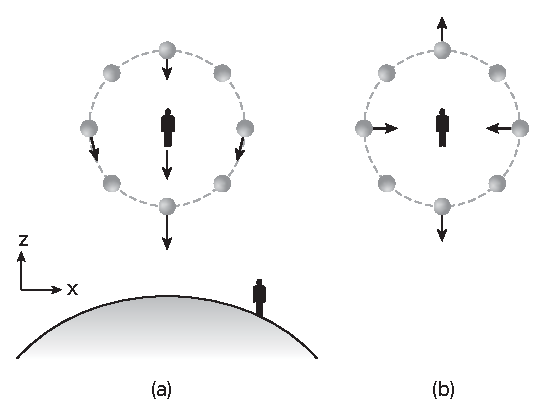
\includegraphics{tidal_of_falling_obj.eps}
	\caption{(a)为地面的观测者看空中的潮汐力,(b)为自由落体观测者参考系}
	\label{tidal_of_falling_obj}
\end{figure}
如果我们将参考系变换到自由落体的物体上,那么我们自然会看到如图\ref{tidal_of_falling_obj}(b)所示的潮汐力,参考系变换即把所有力减去中心粒子所受力即可。如果把自由落体参考系中的潮汐力图像化,即如图\ref{tidal_of_moon}所示,我们可以看到这就是“潮汐”的经典的物理图像。
\begin{figure}[h]
	\centering
	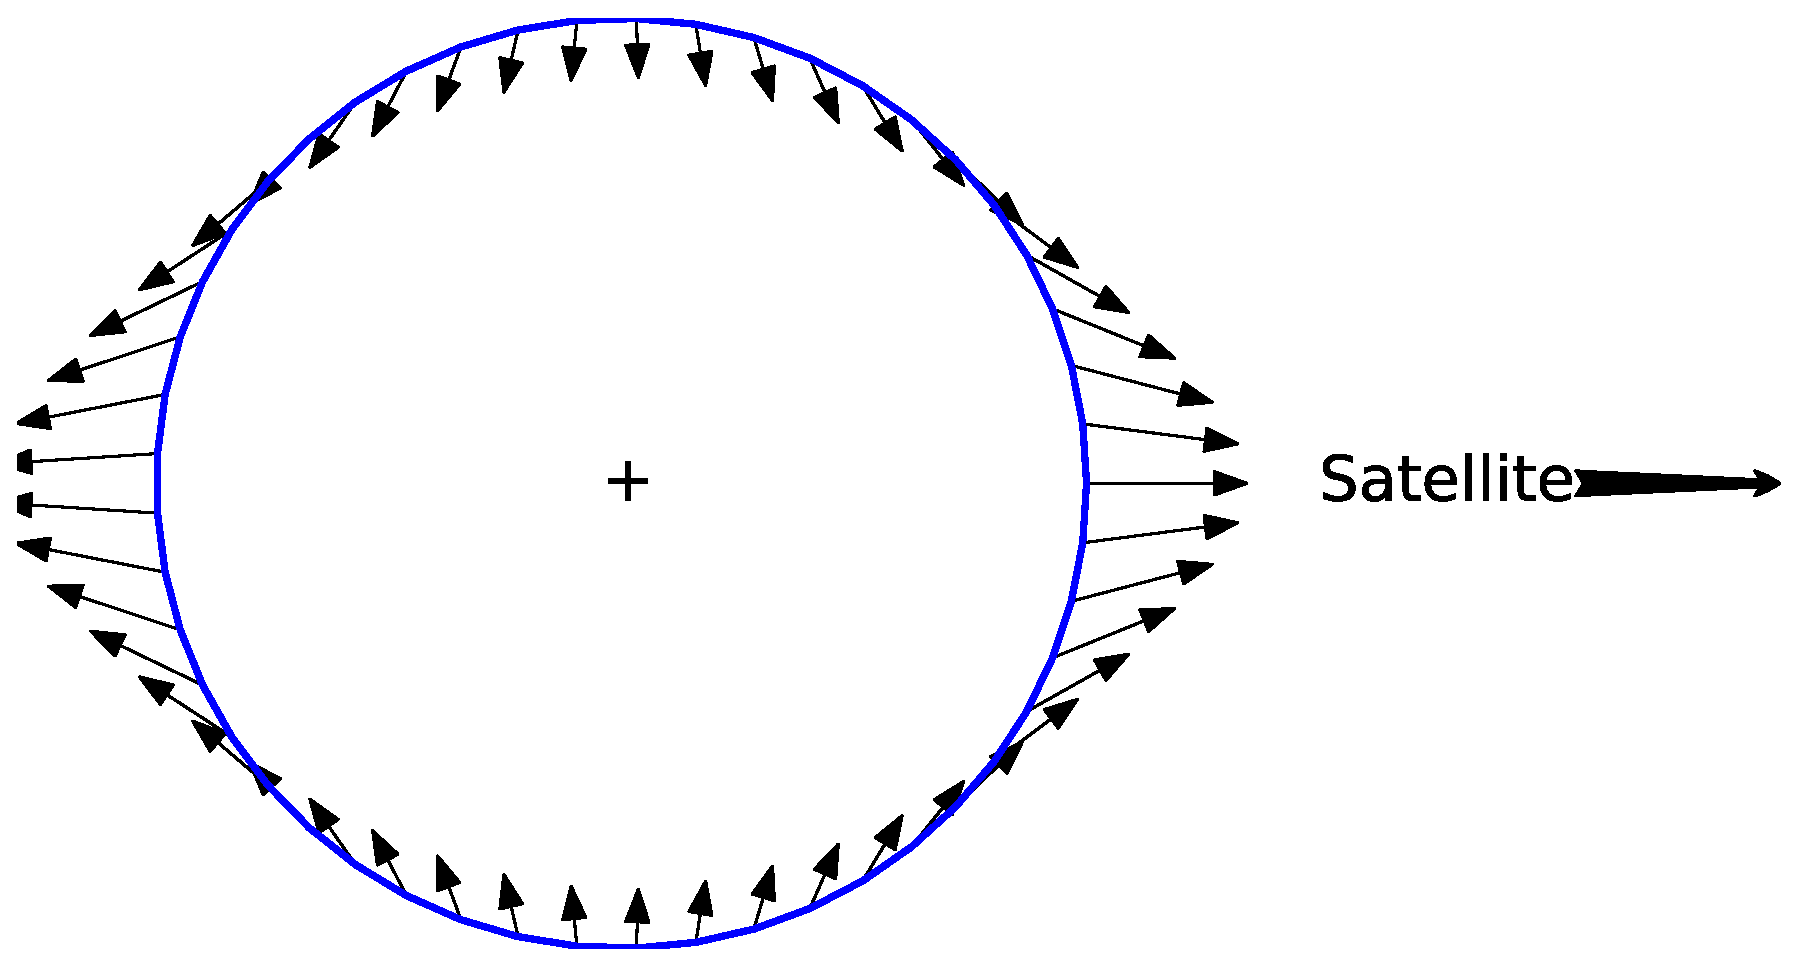
\includegraphics[scale=0.3]{tidal_of_moon.eps}
	\caption{月亮对地球的潮汐力场}
	\label{tidal_of_moon}
\end{figure}
\subsubsection{测地偏移方程}
在广相的框架下,局域的自由粒子总沿着测地线运动,因此如果想要得到引力场的非均匀性,那么我们自然应当考虑两个沿无限接近测地线的自由粒子的运动。考虑两条接近的测地线$\gamma _{0} ,\gamma _{1}$,他们的参数化由$x^{\alpha }( t)$给出,其中$t$为仿射参数。这两条测地线可能是类时,类光或者类空的。类似于经典情景,我们想要获得一个关于这两条测地线的“偏移矢量”并且获得它的方程。如图\ref{geodesic cong}所示,我们在两条测地线中内插一族不相交的测地线,并用参数$s$标记这组测地线(后称测地线汇),即此测地线族为$x^{\alpha }( s,t)$,$s=0$时对应的测地线为$\gamma _{0}$,$s=1$对应的测地线为$\gamma _{1}$。

\begin{figure}
\centering


\tikzset{every picture/.style={line width=0.75pt}} %set default line width to 0.75pt        

\begin{tikzpicture}[x=0.75pt,y=0.75pt,yscale=-1,xscale=1]
%uncomment if require: \path (0,174); %set diagram left start at 0, and has height of 174

%Curve Lines [id:da6599678366291943] 
\draw    (272.01,161.86) .. controls (302.01,132.86) and (267.01,42.86) .. (307.01,12.86) ;
%Curve Lines [id:da7243340632234556] 
\draw    (357.01,161.86) .. controls (387.01,132.86) and (352.01,42.86) .. (392.01,12.86) ;
%Curve Lines [id:da17659953985140864] 
\draw  [dash pattern={on 4.5pt off 4.5pt}]  (293.01,161.86) .. controls (323.01,132.86) and (288.01,42.86) .. (328.01,12.86) ;
%Curve Lines [id:da26658197592140453] 
\draw  [dash pattern={on 4.5pt off 4.5pt}]  (315.01,161.86) .. controls (345.01,132.86) and (310.01,42.86) .. (350.01,12.86) ;
%Curve Lines [id:da03377623956321174] 
\draw  [dash pattern={on 4.5pt off 4.5pt}]  (340.01,161.86) .. controls (370.01,132.86) and (335.01,42.86) .. (375.01,12.86) ;
%Curve Lines [id:da17887242348971033] 
\draw  [dash pattern={on 4.5pt off 4.5pt}]  (252.01,48.39) .. controls (265.01,25.39) and (379.01,24.39) .. (410.01,37.39) ;
%Curve Lines [id:da7269502507510239] 
\draw  [dash pattern={on 4.5pt off 4.5pt}]  (252.01,78.39) .. controls (265.01,55.39) and (379.01,54.39) .. (410.01,67.39) ;
%Curve Lines [id:da8226475847377916] 
\draw  [dash pattern={on 4.5pt off 4.5pt}]  (252.01,110.39) .. controls (265.01,87.39) and (379.01,86.39) .. (410.01,99.39) ;
%Curve Lines [id:da5703454617380816] 
\draw  [dash pattern={on 4.5pt off 4.5pt}]  (252.01,143.39) .. controls (265.01,120.39) and (379.01,119.39) .. (410.01,132.39) ;
%Straight Lines [id:da9561217469497414] 
\draw    (285.01,95.86) -- (283.08,45.86) ;
\draw [shift={(283.01,43.86)}, rotate = 447.8] [color={rgb, 255:red, 0; green, 0; blue, 0 }  ][line width=0.75]    (8.74,-2.63) .. controls (5.56,-1.12) and (2.65,-0.24) .. (0,0) .. controls (2.65,0.24) and (5.56,1.12) .. (8.74,2.63)   ;
%Straight Lines [id:da30666659441265054] 
\draw    (325.01,123.93) -- (390.01,122.96) ;
\draw [shift={(392.01,122.93)}, rotate = 539.14] [color={rgb, 255:red, 0; green, 0; blue, 0 }  ][line width=0.75]    (8.74,-2.63) .. controls (5.56,-1.12) and (2.65,-0.24) .. (0,0) .. controls (2.65,0.24) and (5.56,1.12) .. (8.74,2.63)   ;

% Text Node
\draw (279,2) node [anchor=north west][inner sep=0.75pt]    {$\gamma _{0}$};
% Text Node
\draw (393,0) node [anchor=north west][inner sep=0.75pt]    {$\gamma _{1}$};
% Text Node
\draw (262,42) node [anchor=north west][inner sep=0.75pt]    {$u^{\alpha }$};
% Text Node
\draw (394,107) node [anchor=north west][inner sep=0.75pt]    {$\xi ^{\alpha }$};
% Text Node
\draw (417,33) node [anchor=north west][inner sep=0.75pt]    {$s$};
% Text Node
\draw (235,150) node [anchor=north west][inner sep=0.75pt]    {$s=0$};
% Text Node
\draw (371,150) node [anchor=north west][inner sep=0.75pt]    {$s=1$};


\end{tikzpicture}
\caption{测地线汇$x^{\alpha }( s,t)$}
\label{geodesic cong}
\end{figure}
我们记测地线的切向量为$u^{\alpha } \equiv \partial x^{\alpha } /\partial t$,则我们的测地线方程自然可以写成:
\begin{equation*}
	u^{\alpha }{}_{;\beta } u^{\beta } =0
\end{equation*}
如果我们固定$t$而变动$s$,我们自然得到其他测地线。我们考虑这组测地线的切向量,即$\xi ^{\alpha } \equiv \partial x^{\alpha } /\partial s$。如果我们将$\xi ^{\alpha }$限制到$\gamma _{0}$上,即考虑$\xi ^{\alpha }| _{s=0}$,那么我们可以用此来表示$\gamma _{0}$和$\gamma _{1}$之间的偏差。类比于经典情况,我们自然应当考虑偏差$\xi ^{\alpha }$的“加速度”,即:
\begin{equation*}
	\begin{aligned}
		\frac{\mathrm{D}^{2} \xi ^{\alpha }}{\mathrm{d} t^{2}} & =\frac{\mathrm{D}}{\mathrm{d} t} ( \xi ^{\alpha }{}_{;\beta } u^{\beta } )=( \xi ^{\alpha }{}_{;\beta } u^{\beta } )_{;\gamma } u^{\gamma }
	\end{aligned}
\end{equation*}
在平直时空中,上式应当为$0$,因为平直时空的引力场均匀,两个粒子的测地线应当完全一致。如果上式不为$0$,那自然反映了时空弯曲的二阶效应,即曲率,实际上我们通过计算也可以得出上式正比于黎曼张量。如果我们将上式计算出来就得到了广相框架下的测地偏移方程。由定义:
\begin{equation*}
	u^{\alpha } =\frac{\partial x^{\alpha }}{\partial t} ,\xi ^{\alpha } =\frac{\partial x^{\alpha }}{\partial s} \Rightarrow u^{\alpha }{}_{;\beta } \xi ^{\beta } =\frac{\partial u^{\alpha }}{\partial s} =\frac{\partial ^{2} x^{\alpha }}{\partial t\partial s} =\frac{\partial \xi ^{\alpha }}{\partial t} =\xi ^{\alpha }{}_{;\beta } u^{\beta }
\end{equation*}
实际上,由直觉我们也可以看出$\xi ^{\alpha }$和$u^{\alpha }$是垂直的,如果计算一下:
\begin{equation*}
	\begin{aligned}
		\frac{\mathrm{d}}{\mathrm{d} t} ( \xi ^{\alpha } u_{\alpha } ) & =(\xi ^{\alpha } u_{\alpha } )_{;\beta } u^{\beta } =\xi ^{\alpha }{}_{;\beta } u_{\alpha } u^{\beta } +\xi ^{\alpha } u_{\alpha ;\beta } u^{\beta }\xlongequal{u_{\alpha ;\beta } u^{\beta } =0} u^{\alpha }{}_{;\beta } \xi ^{\beta } u_{\alpha } =\frac{1}{2} (u^{\alpha } u_{\alpha } )_{;\beta } \xi ^{\beta }
	\end{aligned}
\end{equation*}
但由于$u^{\alpha } u_{\alpha } \equiv \varepsilon $为一个常数,因此$\mathrm{d} (\xi ^{\alpha } u_{\alpha } )/\mathrm{d} t=0$。如果我们选取适当的参数,自然可以使$\xi ^{\alpha } u_{\alpha } =0$,因此$\xi ^{\alpha }$处处垂直于$u^{\alpha }$,这也进一步印证了$\xi ^{\alpha }$可以作为测量测地线“偏移”的量。

现在我们来计算“加速度”:
\begin{equation*}
	\begin{aligned}
		\frac{\mathrm{D}^{2} \xi ^{\alpha }}{\mathrm{d} t^{2}} & =(\xi ^{\alpha }{}_{;\beta } u^{\beta } )_{;\gamma } u^{\gamma }\\
		& =(u^{\alpha }{}_{;\beta } \xi ^{\beta } )_{;\gamma } u^{\gamma }\\
		& =u^{\alpha }{}_{;\beta \gamma } \xi ^{\beta } u^{\gamma } +u^{\alpha }{}_{;\beta } \xi ^{\beta }{}_{;\gamma } u^{\gamma }\\
		& =(u^{\alpha }{}_{;\gamma \beta } -R^{\alpha }{}_{\mu \beta \gamma } u^{\mu } )\xi ^{\beta } u^{\gamma } +u^{\alpha }{}_{;\beta } u^{\beta }{}_{;\gamma } \xi ^{\gamma }\\
		& =(u^{\alpha }{}_{;\gamma } u^{\gamma } )_{;\beta } \xi ^{\beta } -\textcolor[rgb]{0.82,0.01,0.11}{u^{\alpha }{}_{;\gamma } u^{\gamma }{}_{;\beta } \xi ^{\beta }} -R^{\alpha }{}_{\mu \beta \gamma } u^{\mu } \xi ^{\beta } u^{\gamma } +\textcolor[rgb]{0.29,0.56,0.89}{u^{\alpha }{}_{;\beta } u^{\beta }{}_{;\gamma } \xi ^{\gamma }}
	\end{aligned}
\end{equation*}
其中第四个等号采用了结论(有时黎曼张量也如此定义):
\begin{equation*}
	u^{\alpha }{}_{;\beta \gamma } -u^{\alpha }{}_{;\gamma \beta } =-R^{\alpha }{}_{\delta \beta \gamma } u^{\delta }
\end{equation*}
但由于测地线方程$u^{\alpha }{}_{;\gamma } u^{\gamma } =0$,因此我们得到了测地偏移方程:
\begin{equation}
	\boxed{\frac{\mathrm{D}^{2} \xi ^{\alpha }}{\mathrm{d} t^{2}} =-R^{\alpha }{}_{\mu \beta \gamma } u^{\mu } \xi ^{\beta } u^{\gamma }}
	\label{geodesic deviation}
\end{equation}
这个方程说明了曲率能造成两条相邻测地线的相对加速度,体现了引力场的“非均匀性”,也正因为此,有时我们也借助式\eqref{geodesic deviation}来定义黎曼张量。

\subsubsection{弱场近似}
一个好的理论必须在非相对论极限下回到牛顿力学,现在我们来看看在弱场近似下测地偏移方程\eqref{geodesic deviation}如何退化到\eqref{GD classic}。在弱场近似下,式\eqref{geodesic deviation}的左侧退化成$\mathrm{d}^{2} /\mathrm{d} t^{2}$,而$u^{\mu }\rightarrow \delta ^{\mu }{}_{0}$,因此我们有:
\begin{equation}
	\frac{\mathrm{d}^{2} \xi ^{\alpha }}{\mathrm{d} t^{2}} =-R^{\alpha }{}_{0\beta 0} \xi ^{\beta }
	\label{GD to cl}
\end{equation}
对比\eqref{GD to cl}和\eqref{GD classic},我们可以发现:
\begin{equation*}
	R^{i}{}_{0j0}\xrightarrow{\text{CL.}} R^{i}{}_{j} =g^{ik} \Phi _{;jk}
\end{equation*}
在球坐标下:
\begin{equation*}
	V( r) =-\frac{GM}{r} \Rightarrow V( r)_{;i} =\frac{GM}{r^{2}} \delta ^{r}{}_{i}
\end{equation*}
为了计算下一步协变导数,我们需要球坐标下的克氏符的$r$分量:\begin{equation*}
	\Gamma ^{r}{}_{\theta \theta } =-r,\Gamma ^{r}{}_{\phi \phi } =-r\sin^{2} \theta 
\end{equation*}

因此我们有:
\begin{equation*}
	V( r)_{;ij} =\partial _{i} \partial _{j} V-\Gamma ^{k}{}_{ij} \partial _{k} V=-\frac{2GM}{r^{3}} \delta ^{r}{}_{i} \delta ^{r}{}_{j} -\Gamma ^{r}{}_{ij}\frac{GM}{r^{2}}
\end{equation*}
故
\begin{equation*}
	R_{11} =-\frac{2GM}{r^{3}} ,R_{22} =\frac{GM}{r} ,R_{33} =\sin^{2} \theta \frac{GM}{r}
\end{equation*}
那么我们需要证明的东西在球坐标下就变成了:
\begin{equation*}
	R^{1}{}_{010}\rightarrow R^{1}{}_{1} =-\frac{2GM}{r^{3}} ,R^{2}{}_{020}\rightarrow R^{2}{}_{2} =\frac{GM}{r^{3}} ,R^{3}{}_{030}\rightarrow R^{3}{}_{3} =\frac{GM}{r^{3}}
\end{equation*}
在牛顿极限下,我们设$g_{\mu \nu } =\eta _{\mu \nu } +h_{\mu \nu }$,对比测地偏移方程和牛顿第二定律我们有:
\begin{equation*}
	h_{00} =-2V\Rightarrow g_{00} =-1+\frac{2GM}{r}
\end{equation*}
那么我们对此度规计算黎曼张量,得到:
\begin{equation*}
	R^{1}{}_{010} =\frac{GM( -3GM+2r)}{( 2GM-r) r^{3}}\xrightarrow{r\gg GM} -\frac{2GM}{r^{3}} ,R^{2}{}_{020} =R^{3}{}_{030} =\frac{GM}{r^{3}} \ 
\end{equation*}
因此测地偏移方程在经典极限下的确退化为了牛顿引力的结果。


\end{document}